\documentclass{beamer}
\usepackage{tikz}
\usepackage{multicol}
\usepackage[style=authoryear,backend=bibtex]{biblatex}
\addbibresource{ref.bib}

\mode<presentation>
{
	\usetheme[progressbar=foot,numbering=fraction,background=light,block=fill]{metropolis}
	\usecolortheme{default}
	\usefonttheme{default}
	\setbeamertemplate{navigation symbols}{}
	\setbeamertemplate{caption}[numbered]
	\setbeamertemplate{frame footer}{Thomas Pappas | ALMA }
}

% Commands for wrapping properly common expressions.
\newcommand{\indeq}[1]{\stackrel{\text{#1}}{=}}
\newcommand{\RightarrowArg}[1]{\stackrel{#1}{\Rightarrow}}
\newcommand{\LeftrightarrowArg}[1]{\stackrel{#1}{\Leftrightarrow}}
\newcommand{\NE}{\mathrm{N.E.}}
\newcommand{\as}{\mathrm{\alpha_s}}
\newcommand{\R}{\mathbb{R}}
\newcommand{\Gm}{\mathcal{G}}
\DeclareMathOperator*{\argmax}{arg\,max}

\title[]{Pricing Games in Heterogeneous Parallel Networks}
\author[Thomas Pappas]{Thomas Pappas}
\institute[ALMA]{
	\begin{columns}
		\column{0.4\textwidth}
		\begin{figure}
			\centering
			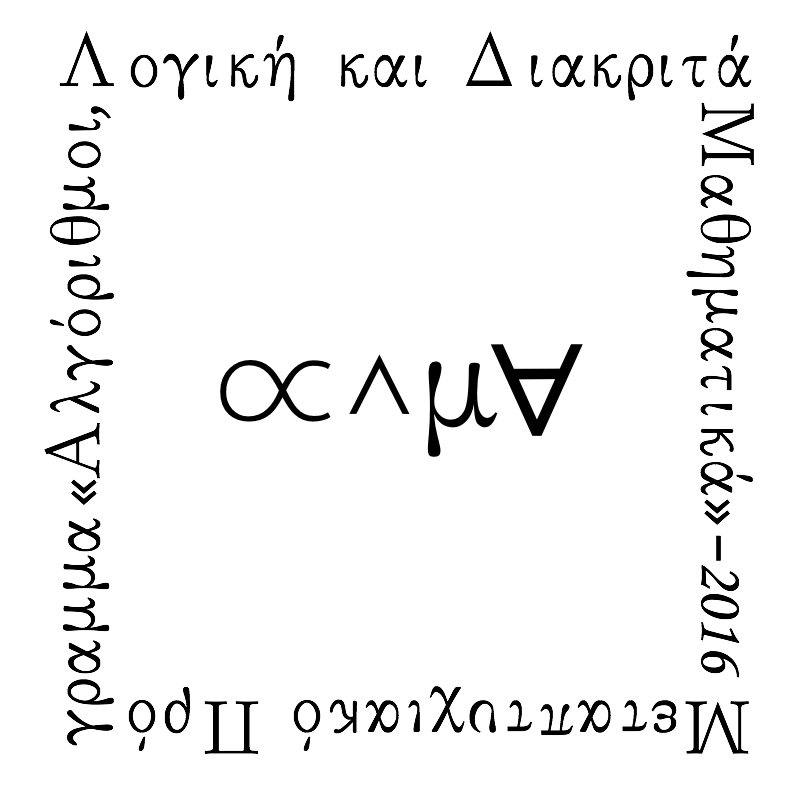
\includegraphics[scale=0.1]{alma.png}
		\end{figure}
		\column{0.5\textwidth}
		ALMA \\
		\tiny{INTER-INSTITUTIONAL GRADUATE PROGRAM \\
			"ALGORITHMS, LOGIC AND DISCRETE MATHEMATICS"}
	\end{columns}
}
\date{\today}

\begin{document}
\AtBeginSection[]{
  \begin{frame}[noframenumbering,plain]
	  \vfill
	  \centering
	  \begin{beamercolorbox}[sep=8pt,center,shadow=true,rounded=true]{title}
	    \usebeamerfont{title}\insertsectionhead\par
	  \end{beamercolorbox}
	  \vfill
  \end{frame}
}


\begin{frame}[noframenumbering,plain]
  \titlepage
\end{frame}

\begin{frame}[noframenumbering,plain]
    \frametitle{Agenda}
    \tableofcontents[hideallsubsections]
\end{frame}


\section{Introduction}

\begin{frame}{History}
	\begin{itemize}
		\item Selfish routing \footcite{pigou1920economics}
		\item Congestion games \footcite{Rosenthal1973ACO}
		\item Wardrop equilibrium \footcite{wardrop_theoretical_1952}
		\item Pricing competition \footcite{10.1287/moor.1060.0231}
		\begin{itemize}
			\item Homogeneous case with toll caps \footcite{Harks_2019}
		\end{itemize}
	\end{itemize}
\end{frame}

\begin{frame}{Our model}
	\begin{center}
		Heterogeneous Non-atomic $n$-link Parallel Network\\
		Toll Congestion Pricing Game
	\end{center}
\end{frame}
\begin{frame}{Our model}
	\begin{center}
		\textbf{Heterogeneous} Non-atomic $n$-link Parallel Network\\
		Toll Congestion \textbf{Pricing} Game
	\end{center}
\end{frame}

\begin{frame}{Our model}
	\;
	\begin{block}{$2$-level game}
		\begin{enumerate}
			\item Shelfish routing game, flow on minimum cost paths
			\item Profit maximisation game for link operators
		\end{enumerate}
	\end{block}
\end{frame}

\begin{frame}{Preliminaries}
	\;
	\begin{block}{Non-atomic $n$-link Parallel Network Game}
		A \textbf{Parallel Network} is a directed graph $G = (\{s, t\}, N)$, where $N = \{1, \dots, n\}$ a set of $n$ parallel $s-t$ links.

		For a \textbf{non-atomic} game, a unit of traffic $[0, 1]$, endowed with Lebesque measure $\lambda$, wishes to travel from $s$ to $t$.

		Traffic creates congestion on links and each \textit{player} $p \in [0, 1]$:
		\begin{itemize}
			\item is selfish and wants to experience minimum congestion
			\item has infinitesimal effect on congestion
		\end{itemize}
	\end{block}

	\begin{center}
		\begin{tikzpicture}[scale=0.8, every node/.style={font=\small}]
			% Nodes
			\node[circle, draw, fill=blue!20, minimum size=0.8cm] (s) at (0, 0) {$s$};
			\node[circle, draw, fill=blue!20, minimum size=0.8cm] (t) at (4, 0) {$t$};

			% Edges
			\draw[->, thick] (s) to[bend left=35] node[midway, above] {$1$} (t);
			\draw[->, thick] (s) to[bend left=10] node[midway, above] {$2$} (t);
			\node[align=center] at (2, 0) {$\vdots$};
			\draw[->, thick] (s) to[bend right=35] node[midway, above] {$n$} (t);
		\end{tikzpicture}
	\end{center}
\end{frame}

\begin{frame}{Preliminaries}
	\;
	\begin{block}{Non-atomic $n$-link Parallel Network Game}
		Flow $f: [0, 1] \rightarrow N$ is a Lebesque measurable function assigning players to links.

		\textit{Flow on paths} $x_i = \lambda(\{p \in [0, 1]: f(p) = i\})$
		\begin{itemize}
			\item $x = (x_i)_{i \in N}$ a (stochastic) vector with $x_i \ge 0$ and $\sum_{i \in N} x_i = 1$
		\end{itemize}
		Congestion on links is represented by affine latency functions $(\ell_i)_{i \in N}$ where $\ell_i \in \mathcal{L}_1$, making congestion on link $i$ equal to $\ell_i(x_i)$.
	\end{block}

	\begin{center}
		\begin{tikzpicture}[scale=1.2, every node/.style={font=\small}]
			% Nodes
			\node[circle, draw, fill=blue!20, minimum size=0.8cm] (s) at (0, 0) {$s$};
			\node[circle, draw, fill=blue!20, minimum size=0.8cm] (t) at (4, 0) {$t$};

			% Edges
			\draw[->, thick] (s) to[bend left=35] node[midway, above] {$\ell_1(x_1)$} (t);
			\draw[->, thick] (s) to[bend left=10] node[midway, above] {$\ell_2(x_2)$} (t);
			\node[align=center] at (2, 0) {$\vdots$};
			\draw[->, thick] (s) to[bend right=35] node[midway, above] {$\ell_n(x_n)$} (t);
		\end{tikzpicture}
	\end{center}
\end{frame}

\begin{frame}{Homogeneous players}
	Links can be tolled by assigning tolls $t \in \R_+^N$.

	Player $p$ experiences on link $i$ total cost $c_i(p) = \ell_i(x_i) + t_i$.
	\begin{definition}
		For a given set of tolls $t$, a flow $x$ is a \textit{Wardrop equilibrium for $t$} if $\forall i, j \in N$ with $x_i > 0$ it holds that
		\begin{equation*}
			\ell_i(x_i) + t_i \leq \ell_j(x_j) + t_j
		\end{equation*}
	\end{definition}
	Links with $x_i > 0$ have $\ell_i(x_i) + t_i = K$ for some $K > 0$.

	Wardrop equilibrium always exits and is unique\footcite{??}, denote it by $x(t)$.
\end{frame}

\begin{frame}{Homogeneous players}
	\begin{lemma}[variational inequality\footcite{dafermos1973toll}]
		A flow $x$ is a Wardrop equilibrium for $t$ if and only if for all feasible flows $x^\prime$,
		\[\sum_{i \in N} (\ell_i(x_i) + t_i) \cdot (x_i - x_i^\prime) \leq 0\]
	\end{lemma}
	Equilibrium is indifferent to uniform variations of tolls ($t^\prime = t + c$) or (affine) latencies.
\end{frame}

\begin{frame}{Heterogeneous players}
	Players value time-money differently, so add weight $\alpha$ to money.
	\begin{block}{Distribution function $\alpha: [0, 1] \rightarrow [0, +\infty]$}
		\begin{itemize}
			\item players are ordered w.r.t. sensitivity
			\item $\alpha$ is non-decreasing
		\end{itemize}
	\end{block}
	Player $p$ experiences on link $i$ total cost $c_i(p) = \ell_i(x_i) + \alpha(p) \cdot t_i$.
	\begin{definition}
		For a given set of tolls $t$, a flow $x$ is a \textit{Nash equilibrium for $t$} if for all players $p \in [0, 1]$ and $\forall i \in N$ it holds that
		\begin{equation*}
			c_{f(p)}(p) \leq c_i(p)
		\end{equation*}
	\end{definition}
\end{frame}

\begin{frame}{Heterogeneous players}
	\begin{example}
		Let $([2], \ell, \alpha)$ with $\ell_1(x) = 2x, \ell_2(x) = x + 1$ and $\alpha(p) = p + 1$.
	\end{example}
	\begin{center}
		\begin{tikzpicture}[scale=1.4, every node/.style={font=\small}]
			% Nodes
			\node[circle, draw, fill=blue!20, minimum size=0.8cm] (s) at (0,0) {$s$};
			\node[circle, draw, fill=blue!20, minimum size=0.8cm] (t) at (4,0) {$t$};

			% Links
			\draw[->, thick] (s) to[bend left=35] node[midway, above] {$2x$} (t);
			\draw[->, thick] (s) to[bend right=35] node[midway, below] {$x + 1$} (t);

			% Description
			%\node[align=center] at (2, -2) {Network of Example};
		\end{tikzpicture}
	\end{center}
	$x(0) = \left(\frac23, \frac13\right), \; x(3, 2) = \left(\frac14, \frac34\right)$
\end{frame}

\begin{frame}{Heterogeneous players}
	Nash equilibrium for $t$ always exists\footcite{1973JSP.....7..295S} and is unique\footcite{MILCHTAICH1996111}, again denote it by $x(t)$.
\end{frame}

\begin{frame}{Pricing competition (2\textsuperscript{nd} level)}
	Links are owned by agents who compete for profit.
	\begin{block}{Profit}
		For given set of tolls $t \in \R_+^N$, link operator $i$ gains profit
		\[\Pi_i(t) = x_i(t) \cdot t_i\]
	\end{block}

	\begin{block}{Best response}
		For fixed tolls assignments from remaining link operators $t_{-i} = t \setminus \{t_i\}$, link operator $i$ will try and maximise their profit
		\[B_i(t_{-i}) = \argmax_{t_i \ge 0} \Pi(t_i, t_{-i})\]
	\end{block}
\end{frame}

\begin{frame}{Pricing competition (2\textsuperscript{nd} level)}
	\begin{block}{Nash Equilibrium}
		A given set of tolls $t$ is a \textit{Nash Equilibrium for the pricing game} if $\forall i \in N$ and $\forall t_i^\prime \in \R_+$
		\[\Pi_i(t_i, t_{-i}) \geq \Pi_i(t_i^\prime, t_{-i})\]
	\end{block}
	\begin{block}{Nash Equilibrium}
		A given set of tolls $t$ is a \textit{Nash Equilibrium for the pricing game} if
		$\forall i \in N$ we have $|B_i(t_{-i})| = 1$ and
		\[t = (B_i(t_{-i}))_{i \in N}\]
	\end{block}
\end{frame}

\begin{frame}{Game equivalence}
	\begin{definition}[Game equivalence]
		Let $\Gm_1, \Gm_2$ be two $n$-link Network Congestion Games.
		$\Gm_1$ and $\Gm_2$ are called \textbf{equivalent} if and only if for all tolls $t \in \R_+$ it holds that $x^{(1)}(t) = x^{(2)}(t)$, with $x^{(1)}(t), x^{(2)}(t)$ being the Nash Equilibria for $t$ in $\Gm_1, \Gm_2$ respectively.
	\end{definition}
	The two pricing competition games played on two equivalent network congestion games are identical.
\end{frame}


\section{Heterogeneous players}

\begin{frame}{Heterogeneous players}
	\begin{lemma}
		For $\Gm = (N, \ell, \alpha)$ with tolls $t$ and flow $x(t)$ the Nash equilibrium for $t$, it holds for all $i, j \in N$ with $x_i(t), x_j(t) > 0$ that
		\begin{enumerate}[(i)]
			\item $\ell_i(x_i(t)) < \ell_j(x_j(t))$ iff $t_i > t_j$
			\item $\ell_i(x_i(t)) = \ell_j(x_j(t))$ iff $t_i = t_j$
			\item $\ell_i(x_i(t)) > \ell_j(x_j(t))$ iff $t_i < t_j$
		\end{enumerate}
	\end{lemma}
	\begin{proof}
		Assume $\ell_i(x_i(t)) < \ell_j(x_j(t))$ and $t_i < t_j$ for some $i, j \in N$.
		Then for \textbf{all} players $c_i(p) < c_j(p)$ so $x_j(t) > 0$ is a contradiction.
	\end{proof}
\end{frame}

\begin{frame}{Heterogeneous players}
	Latencies are viewed the same for all players.

	Toll order is the same for all players.

	Tolls define an ordering of the $N$ links where
	\begin{itemize}
		\item $t_1 \ge t_2 \ge \dots \ge t_n$
		\item $\ell_1(x_1(t)) \le \ell_2(x_2(t)) \le \dots \le \ell_n(x_n(t))$
		\item for player representatives from each link $p_1, p_2, \dots, p_n$ we also get $\alpha(p_1) \le \alpha(p_2) \le \dots \le \alpha(p_n)$
	\end{itemize}
	Ordering is unique only when the toll (and therefore also latency) inequalities are strict.
\end{frame}


\section{Sensitivity split}

\begin{frame}{Sensitivity split}
	In a heterogeneous game, in practice, each flow user plays a different game.

	In example ?? the users are organised around the one for which $c_1(p) = c_2(p)$.

	We need the notion of the money-sensitivity value for which two link costs are equal.
\end{frame}

\begin{frame}{Sensitivity split}
	\begin{definition}
		Let $(N, \ell, \alpha)$ a heterogeneous parallel game, tolls $t$ where $t_i \ne t_j$ for links $i, j \in N$ and $x(t)$ the Nash equilibrium for $t$.
		We define the \textit{money sensitivity split function} $\as^{(i, j)}: \{t \in \R_+^N|t_i \ne t_j\} \rightarrow (0, +\infty)$ as
		\[\as^{(i, j)}(t) = \frac{\ell_j(x_j(t)) - \ell_i(x_i(t))}{t_i - t_j}\]
	\end{definition}
	If $t_i = t_j \Leftrightarrow \ell_i(x_i) = \ell_j(x_j)$ then $c_i(p) = c_j(p)$ for \textbf{all} flow users.
\end{frame}

\begin{frame}{Sensitivity split}
	If $t_i \ne t_j$ then assume w.l.o.g. $t_i > t_j \Leftrightarrow \ell_i(x_i) < \ell_j(x_j)$.\\
	Low money-sensitive players will use link $i$.\\
	High money-sensitive players will use link $j$.

	\begin{table}[h!]
		\centering
		\caption{Summary of properties for the sensitivity split.}
		\begin{tabular}{| c || c | c |}
			\hline
			& \textbf{lower split} & \textbf{upper split} \\ \hline
			$\alpha$ & $\alpha(p) \le \as^{(i, j)}(t)$ & $\alpha(p) \ge \as^{(i, j)}(t)$ \\ \hline
			link & low-latency, high-toll & high-latency, low-toll \\ \hline
			sensitivity & time $\ge$ money & time $\le$ money \\ \hline
		\end{tabular}
		\label{table:split_summary}
	\end{table}
\end{frame}

\begin{frame}{Sensitivity split}
	\begin{definition}
		\label{definition:alpha_flow_sets}
		Let $(N, \ell, \alpha)$ a heterogeneous parallel game, tolls $t$ and $x(t)$ the Nash equilibrium for $t$.
		We define as $A_i(t)$ the set of all possible $\alpha(p)$ values of players $p$ using link $i$ in the Nash equilibrium for $t$.
		We define a set function $A_i: \R_+^{|N|} \rightarrow \mathcal{P}(\R_+)$, where $\mathcal{P}(\R_+)$ is the powerset of $\R_+$, such that
		\[A_i(t) = \{\alpha(p) | f(p) = j \wedge t_j = t_i\}\]
	\end{definition}

	Notice that with this definition it follows that $A_i(0)$ is the entire domain of $\alpha$ for any $i \in N$.
\end{frame}

\begin{frame}{Sensitivity split}
	\begin{lemma}
		Let $(N, \ell, \alpha)$ a heterogeneous parallel game and tolls $t$ where $t_i \ne t_j$ and $x_i(t), x_j(t) > 0$ for some links $i, j \in N$.
		Then the following hold:
		\begin{enumerate}[(i)]
			\item $\as^{(i, j)}(t) > 0$
			\item $\as^{(i, j)}(t) \in [\alpha(0), \alpha(1)]$
			%\item if $\as^{(i, j)}(t) < \alpha(0)$ (or $\as^{(i, j)}(t) > \alpha(1)$) then $x(t) = (0, 1)$ (or $(1, 0)$)
			\item if $\ell_i(x_i(t)) < \ell_j(x_j(t))$ then
			$\sup A_i(t) \le \as^{(i, j)}(t) \le \inf A_j(t)$
		\end{enumerate}
	\end{lemma}
\end{frame}

\begin{frame}{Sensitivity split | Monotonicity}
	\begin{lemma}
		Let $(N, \ell, \alpha)$ a heterogeneous parallel game and tolls $t, t^\prime$ such that for some links $i, j \in N$ it holds that $t_i \ne t_j, t_i^\prime \ne t_j^\prime$ and $t_k = t_k^\prime$ $\forall k \in N \setminus \{i, j\}$.
		If $x_i(t), x_j(t), x_i(t^\prime), x_j(t^\prime) > 0$ and $\frac{t_i - t_j}{t_i^\prime - t_j^\prime} > 0$, then:
		\begin{enumerate}[(i)]
			\item if $\frac{t_i - t_j}{t_i^\prime - t_j^\prime} \le 1$ then $\as^{(i, j)}(t) \ge \as^{(i, j)}(t^\prime)$
			\item if $\frac{t_i - t_j}{t_i^\prime - t_j^\prime} \ge 1$ then $\as^{(i, j)}(t) \le \as^{(i, j)}(t^\prime)$
		\end{enumerate}
	\end{lemma}
\end{frame}

\begin{frame}{Sensitivity split | Monotonicity}
	\begin{proof}
		We prove $(i)$ and $(ii)$ follows symmetrically.\\
		If $x(t) = x(t^\prime)$ then the property follows from the definition of $\as$.
		If $x(t) \ne x(t^\prime)$ then assume w.l.o.g. that $x_i(t) > x_i(t^\prime)$, so a player $p$ moved from $i$ to $j$ between $t$ and $t^\prime$.
		\[\inf A_j(t^\prime) \le \alpha(p) \le \sup A_i(t)\]
		Applying the previous lemma gives us
		\[\as^{(i, j)}(t^\prime) \le \inf A_j(t^\prime) \le \sup A_i(t) \le \as^{(i, j)}(t)\]
	\end{proof}
\end{frame}

\begin{frame}{Sensitivity split | Limits}
	\begin{lemma}
		Let $(N, \ell, \alpha)$ a heterogeneous parallel game and tolls $t$ where $t_i \ne t_j$ and $x_i(t), x_j(t) > 0$ for some links $i, j \in N$.
		Then:
		\begin{enumerate}[(i)]
			\item
			\begin{flalign*}
				\lim_{|t_i - t_j| \rightarrow +\infty}\as^{(i, j)}(t) &= 0 &
			\end{flalign*}
			\item
			\begin{flalign*}
				\lim_{t_i - t_j \rightarrow 0^+} \as^{(i, j)}(t) &= \limsup_{t_i - t_j \rightarrow 0^+} A_i(t) &
			\end{flalign*}
		\end{enumerate}
	\end{lemma}
\end{frame}

\begin{frame}{Sensitivity split | Limits}
	\begin{proof}
		$ $
		\begin{enumerate}[(i)]
			\item For $L = \max\{\ell_i(1) - \ell_j(0), \ell_j(1) - \ell_i(0)\}$ we find
			\begin{flalign*}
				\lim_{|t_i - t_j| \rightarrow +\infty}|\as^{(i, j)}(t)| &= \lim_{|t_i - t_j| \rightarrow +\infty}\frac{|\ell_i(x_i(t)) - \ell_j(x_j(t))|}{|t_i - t_j|}\\
				&\le \lim_{|t_i - t_j| \rightarrow +\infty}\frac{L}{|t_i - t_j|} = 0
			\end{flalign*}
		\end{enumerate}
	\end{proof}
\end{frame}

\begin{frame}{Sensitivity split | Limits}
	\begin{proof}
		$ $
		\begin{enumerate}[(ii)]
			\item ...
		\end{enumerate}
	\end{proof}
\end{frame}

\begin{frame}{Sensitivity split}
	\begin{figure}
		\centering
		\begin{tikzpicture}[x=2cm, y=2cm, every node/.style={font=\small}]
			% Axes
			\draw[->] (0,0) -- (-1.1,0);
			\draw[->] (0,0) -- (2.1,0) node[right] {$t_1 - t_2$};
			\draw[->] (0,0) -- (0,2.2) node[above] {$\as(t)$};

			% Tick marks
			\draw (-1,0) -- (-1,-0.05) node[below] {$-1$};
			\draw (0,0) -- (0,-0.05) node[below] {$t_2$};
			\draw (2,0) -- (2,-0.05) node[below] {$2$};
			\draw (0,2) -- (-0.05, 2) node[left] {$2$};
			\draw (0,4/3) -- (0.05,4/3) node[right] {$4/3$};
			\draw (0,5/3) -- (-0.05,5/3) node[left] {$5/3$};
			\draw (0,1) -- (-0.05,1) node[left] {$1$};

			% Function graph
			%\draw[thick] (-1,1) -- (0,4/3);
			%\draw[thick] (0,5/3) -- (2,1);
			\draw[thick,domain=-1:0] plot (\x,{4/(3-\x)});
			\draw[thick,domain=0:2] plot (\x,{5/(3+\x)});

			% Dots
			\fill[white] (0,4/3) ellipse (0.03 and 0.03);
			\draw[black] (0,4/3) ellipse (0.03 and 0.03);
			\fill[white] (0,5/3) ellipse (0.03 and 0.03);
			\draw[black] (0,5/3) ellipse (0.03 and 0.03);
		\end{tikzpicture}
		\caption{Split function of Example}
		\label{figure:alpha_simple:split_example}
	\end{figure}
\end{frame}

\begin{frame}{Sensitivity split | Upper bound}
	We observe that $\as$ might never take some upper values of $\alpha$.\\
	Are then those values relevant?

	\begin{theorem}
		Let $\Gm_1 = (N, \ell, \alpha^{(1)})$ and $\Gm_2 = (N, \ell, \alpha^{(2)})$ be two heterogeneous parallel games and $x(0) = x^{(1)}(0) = x^{(2)}(0)$ the (equal) flow on paths for $t = 0$.
		If $\alpha^{(1)}$ and $\alpha^{(2)}$ are such that
		\[\alpha^{(1)}(p) = \alpha^{(2)}(p), \forall p: p < 1 - \min_{i \in N}\{x_i(0)\}\]
		then $\Gm_1$ and $\Gm_2$ are equivalent.
	\end{theorem}
\end{frame}

\begin{frame}{Sensitivity split | Upper bound}
	\begin{proof}
		...
	\end{proof}
\end{frame}

\begin{frame}{Sensitivity split | Upper bound}
	For the Example we have
	\[\max\{x_1(0), x_2(0)\} = \max\{2/3, 1/3\} = 2/3\]
	so if we used a distribution function such as
	\[
		\alpha(p) =
		\begin{cases}
			p + 1 & p \le 2/3 \\
			\mathrm{e}^p & p > 2/3
		\end{cases}
	\]
	then $\as(t)$ would remain the same for all $t \in \R_+^n$
\end{frame}


\section{Pseudo-heterogeneous Pricing Games}

\begin{frame}{Heterogeneous Pricing Games}
	Zero money sensitivity creates issues.
	\begin{lemma}
		Let $(N, \ell, \alpha)$ where $\exists \epsilon > 0: \alpha(p) = 0 \; \forall p < \epsilon$.
		Let $i \in N$ be a link for which $\ell_i(0) = \min_{j \in N} \ell_i(0)$.
		Then $B_i(t_{-i})$ is unbounded for all $t_{-i} \in \R_+^{|N| - 1}$.
	\end{lemma}
	\begin{proof}
		$\ell_i(0) = \min_{j \in N} \ell_i(0)$, ensures link $i$ will always have flow

		$i$ can select $t_i > \max t_{-i}$ to make link $i$ the lowest-latency link, populated exclusively by players with $\alpha(p) = 0$

		We fix $t_i^\prime$ and we see that
		\[
			\lim_{t_i \rightarrow +\infty} \Pi_i(t_i, t_{-i}) \ge \lim_{t_i \rightarrow +\infty} x_i^\prime(t_i^\prime, t_{-i})t_i = +\infty
		\]
		making in turn $B_i(t_{-i}) = +\infty$.
	\end{proof}
\end{frame}

\begin{frame}{Pseudo-heterogeneous Pricing Games}
	Consider cases where $\alpha(p) = c$ for some $c \in \R_+$.
	\[
		\sum_{i \in N} (\ell(x_i(t)) + c t_i) \cdot (x_i(t) - x_i) \leq 0
	\]

	\begin{lemma}
		Let $\Gm_1 = (N, \ell^{(1)}, c)$ a heterogeneous pricing game with distribution function $\alpha(p) = c$ for some $c > 0$ and $\Gm_2 = (N, \ell^{(2)}, 1)$ a homogeneous pricing game with latencies $\ell^{(2)} = \frac{\ell^{(1)}}{c}$ for the same $c$.
		Then the two games are equivalent.
	\end{lemma}
	We will call such games \textit{pseudo-heterogeneous}.

	Latency-sensitivity relation is lost for general $\alpha$
\end{frame}

\begin{frame}{Pseudo-heterogeneous Pricing Games}
	\begin{figure}
		\centering
		\begin{tikzpicture}[x=3.4cm, y=3.4cm, every node/.style={font=\small}]
			% Axes
			\draw[->] (0,0) -- (-1.1,0);
			\draw[->] (0,0) -- (2.1,0) node[right] {$t_1 - t_2$};
			\draw[->] (0,0) -- (0,1.1) node[above] {$x_1(t)$};

			% Tick marks
			\draw (-1,0) -- (-1,-0.05) node[below] {$-1$};
			\draw (-1/3,0) -- (-1/3,-0.05) node[left=9,below] {$-\frac13$};
			\draw (-1/4,0) -- (-1/4,-0.05) node[right=3,below] {$-\frac14$};
			\draw (0,0) -- (0,-0.05) node[below] {$t_2$};
			\draw (2/4,0) -- (2/4,-0.05) node[below] {$\frac12$};
			\draw (2/3,0) -- (2/3,-0.05) node[below] {$\frac23$};
			\draw (2,0) -- (2,-0.05) node[below] {$2$};
			\draw (0,1) -- (0.05,1) node[right] {$1$};
			\draw (0,2/3) -- (-0.05,2/3) node[left] {$\frac23$};

			% Flow function graphs
			\draw[thick, blue!33] (-1,1) -- (2,0) node[above, black] {$\alpha = 1$};
			\draw[thick, blue!66] (-1/3,1) -- (2/3,0) node[above right, black] {$\alpha = 3$};
			\draw[thick, blue!100] (-1/4,1) -- (2/4,0) node[black] at (0.2,0.17) {$\alpha = 4$};
		\end{tikzpicture}
		\caption{Flow function for link $1$ of Example for $\alpha(p) = 1, 3, 4$.}
	\end{figure}
\end{frame}

\begin{frame}{Pseudo-heterogeneous Pricing Games}
	\begin{lemma}
		Let $\Gm_1 = (N, \ell, c_1)$ and $\Gm_2 = (N, \ell, c_2)$ two heterogeneous pricing games with $\alpha^{(1)}(p) = c_1 > 0$, $\alpha^{(2)}(p) = c_2 > 0$, then
		\begin{enumerate}[$(i)$]
			%\item $x^{(1)}(0) = x^{(2)}(0)$
			\item $x^{(1)}(c_2 t) = x^{(2)}(c_1 t)$
			\item $\frac{\Pi_i^{(1)}(c_2 t)}{\Pi_i^{(2)}(c_1 t)} = \frac{c_2}{c_1}$
			\item $\frac{B_i^{(1)}(c_2t_{-i})}{B_i^{(2)}(c_1 t_{-i})} = \frac{c_2}{c_1}$
		\end{enumerate}
	\end{lemma}
\end{frame}

\begin{frame}{Pseudo-heterogeneous Pricing Games}
	\begin{lemma}
		Let $\Gm_1 = (N, \ell, c_1)$ and $\Gm_2 = (N, \ell, c_2)$ two heterogeneous pricing games with $\alpha^{(1)}(p) = c_1 > 0$, $\alpha^{(2)}(p) = c_2 > 0$.\\
		Let $t^{*(1)}, t^{*(2)}$ the Nash Equilibria for the pricing games in $\Gm_1$ and $\Gm_2$.
		Then
		\begin{enumerate}[$(i)$]
			\item $\frac{t^{*(1)}}{t^{*(2)}} = \frac{c_2}{c_1}$
			\item $x^{(1)}(t^{*(1)}) = x^{(2)}(t^{*(2)})$
		\end{enumerate}
	\end{lemma}
	Nash Equilibrium always at the same flow.
\end{frame}

\section{Step distribution functions}

\begin{frame}{Step distribution functions}
	We will limit our model to instances with $2$ links.

	In $2$-link games, $\as(t)^{(1, 2)} = \as(t)$.

	There always exists an $\alpha$ value for which the two link costs are equal.
\end{frame}

\begin{frame}{Step distribution functions}
	\begin{lemma}
		Let $\Gm_1 = ([2], \ell, \alpha^{(1)})$ a heterogeneous game, $t \ne 0$ a given set of tolls and $x^{(1)}(t)$ the Nash equilibrium for $t$.
		Now let $\Gm_2 = ([2], \ell, \as^{(1)}(t))$ a pseudo-heterogeneous game with latency functions the same as $\Gm_1$ and fixed distribution function $\alpha^{(2)}(p) = \as^{(1)}(t)$.
		Then
		\begin{enumerate}[$(i)$]
			\item $x^{(1)}(t) = x^{(2)}(t)$
			\item $\Pi_i^{(1)}(t) = \Pi_i^{(2)}(t)$ for each respective link operator $i$
		\end{enumerate}
	\end{lemma}
\end{frame}

\begin{frame}{Step distribution functions}
	\begin{example}
		Let $([2], \ell, \alpha)$ a heterogeneous pricing game with latency functions $\ell_1(x) = 2x, \ell_2(x) = x + 1$ and distribution function $\alpha$ such that
		\begin{align*}
			\alpha(p) =
			\begin{cases}
				1 & p \le \tfrac15 \\
				3 & p \in \left(\tfrac15, \tfrac12\right) \\
				4 & p \ge \tfrac12
			\end{cases}&
		\end{align*}
	\end{example}

	\begin{center}
		\begin{multicols}{2}
			% Left Column: Network Graph
			\begin{tikzpicture}[scale=1.4, every node/.style={font=\small}]
				% Nodes
				\node[circle, draw, fill=blue!20, minimum size=0.8cm] (s) at (0,0) {$s$};
				\node[circle, draw, fill=blue!20, minimum size=0.8cm] (t) at (4,0) {$t$};

				% Links
				\draw[->, thick] (s) to[bend left=35] node[midway, above] {$2x$} (t);
				\draw[->, thick] (s) to[bend right=35] node[midway, below] {$x + 1$} (t);

				% Description
				\node[align=center] at (2, -2) {Network of Example};
			\end{tikzpicture}

			% Right Column: Distribution function Graph
			\begin{tikzpicture}[x=3cm, y=0.7cm, every node/.style={font=\small}]
				% Axes
				\draw[->] (0,0) -- (1.2,0) node[right] {$p$};
				\draw[->] (0,0) -- (0,4.2) node[above] {$\as(p)$};

				% Tick marks
				\draw (0,0) -- (0,-0.05) node[below] {$0$};
				\draw (0.2,0) -- (0.2,-0.05) node[below] {$\frac15$};
				\draw (0.5,0) -- (0.5,-0.05) node[below] {$\frac12$};
				\draw (1,0) -- (1,-0.05) node[below] {$1$};
				\draw (0,1) -- (-0.05,1) node[left] {$1$};
				\draw (0,3) -- (-0.05,3) node[left] {$3$};
				\draw (0,4) -- (-0.05,4) node[left] {$4$};

				% Function graph
				\draw[thick] (0,1) -- (0.2,1);
				\draw[thick] (0.2,3) -- (0.5,3);
				\draw[thick] (0.5,4) -- (1,4);

				% Closed / Open dots
				\fill[white] (0.2,1) ellipse (0.014 and 0.06);
				\draw[black] (0.2,1) ellipse (0.014 and 0.06);
				\fill[black] (0.2,3) ellipse (0.014 and 0.06);
				\draw[black] (0.2,3) ellipse (0.014 and 0.06);
				\fill[black] (0.5,3) ellipse (0.014 and 0.06);
				\draw[black] (0.5,3) ellipse (0.014 and 0.06);
				\fill[white] (0.5,4) ellipse (0.014 and 0.06);
				\draw[black] (0.5,4) ellipse (0.014 and 0.06);

				% Description
				\node[align=center] at (0.7, -1.7) {Distribution function of Example};
			\end{tikzpicture}
		\end{multicols}
	\end{center}
\end{frame}

\begin{frame}{Step distribution functions}
	\begin{figure}
		\centering
		\begin{tikzpicture}[x=3.4cm, y=1cm, every node/.style={font=\small}]
			% Axes
			\draw[->] (0,0) -- (-1.1,0);
			\draw[->] (0,0) -- (2.1,0) node[right] {$t_1 - t_2$};
			\draw[->] (0,0) -- (0,4.4) node[above] {$\as(t)$};

			% Tick marks
			\draw (-1,0) -- (-1,-0.05) node[below] {$-1$};
			\draw (-2/5,0) -- (-2/5,-0.05) node[below] {$-\frac25$};
			\draw (-2/15,0) -- (-2/15,-0.05) node[below] {$-\frac{2}{15}$};
			\draw (0,0) -- (0,-0.05) node[below] {$t_2$};
			\draw (1/8,0) -- (1/8,-0.05) node[below] {$\frac18$};
			\draw (1/6,0) -- (1/6,-0.05) node[below] {$\frac16$};
			\draw (7/15,0) -- (7/15,-0.05) node[below] {$\frac{7}{15}$};
			\draw (7/5,0) -- (7/5,-0.05) node[below] {$\frac75$};
			\draw (2,0) -- (2,-0.05) node[below] {$2$};
			\draw (0,1) -- (-0.05,1) node[left] {$1$};
			\draw (0,3) -- (0.05,3) node[right] {$3$};
			\draw (0,4) -- (-0.05,4) node[left] {$4$};

			% Function graph
			% Left side
			\draw[thick] (-1,1) -- (-2/5,1);
			\draw[thick] (-2/5,1) -- (-2/15,3);
			\draw[thick] (-2/15,3) -- (0,3);
			% Right side
			\draw[thick] (0,4) -- (1/8,4);
			\draw[thick] (1/8,4) -- (1/6,3);
			\draw[thick] (1/6,3) -- (7/15,3);
			\draw[thick] (7/15,3) -- (7/5,1);
			\draw[thick] (7/5,1) -- (2,1);

			% Dots
			\fill[white] (0,3) ellipse (0.02 and 0.066);
			\draw[black] (0,3) ellipse (0.02 and 0.066);
			\fill[white] (0,4) ellipse (0.02 and 0.066);
			\draw[black] (0,4) ellipse (0.02 and 0.066);
		\end{tikzpicture}
		\caption{Split function of Example}
		\label{figure:alpha_step:split}
	\end{figure}
\end{frame}

\begin{frame}{Step distribution functions}
	\begin{figure}
		\centering
		\begin{tikzpicture}[x=3.4cm, y=3.4cm, every node/.style={font=\small}]
			% Axes
			\draw[->] (0,0) -- (-1.1,0);
			\draw[->] (0,0) -- (2.1,0) node[right] {$t_1 - t_2$};
			\draw[->] (0,0) -- (0,1.1) node[above] {$x_1(t)$};

			% Tick marks
			\draw (-1,0) -- (-1,-0.05) node[below] {$-1$};
			\draw (-2/5,0) -- (-2/5,-0.05) node[below] {$-\frac25$};
			\draw (-2/15,0) -- (-2/15,-0.05) node[below] {$-\frac{2}{15}$};
			\draw (0,0) -- (0,-0.05) node[below] {$t_2$};
			\draw (1/8,0) -- (1/8,-0.05) node[below] {$\frac18$};
			\draw (1/6,0) -- (1/6,-0.05) node[below] {$\frac16$};
			\draw (7/15,0) -- (7/15,-0.05) node[below] {$\frac{7}{15}$};
			\draw (7/5,0) -- (7/5,-0.05) node[below] {$\frac75$};
			\draw (2,0) -- (2,-0.05) node[below] {$2$};
			\draw (0,1) -- (-0.05,1) node[left] {$1$};
			\draw (0,4/5) -- (0.05,4/5) node[right] {$\frac45$};
			\draw (0,2/3) -- (-0.05,2/3) node[left] {$\frac23$};
			\draw (0,1/2) -- (-0.05,1/2) node[left] {$\frac12$};
			\draw (0,1/5) -- (-0.05,1/5) node[left] {$\frac15$};

			% Function graph
			% Base flow functions
			\draw[gray,dashed, very thin] (-1,1) -- (2,0);
			\draw[gray,dashed, very thin] (-1/3,1) -- (2/3,0);
			\draw[gray,dashed, very thin] (-1/4,1) -- (2/4,0);

			% Left side
			\draw[thick] (-1,1) -- (-2/5,4/5);
			\draw[thick] (-2/5,4/5) -- (-2/15,4/5);
			\draw[thick] (-2/15,4/5) -- (0,2/3);
			% Right side
			\draw[thick] (0,2/3) -- (1/8,1/2);
			\draw[thick] (1/8,1/2) -- (1/6,1/2);
			\draw[thick] (1/6,1/2) -- (7/15,1/5);
			\draw[thick] (7/15,1/5) -- (7/5,1/5);
			\draw[thick] (7/5,1/5) -- (2,0);
		\end{tikzpicture}
		\caption{Flow function for link $1$ of Example}
		\label{figure:alpha_step:flow}
	\end{figure}
\end{frame}

\begin{frame}{Step distribution functions}
	Notice that when $x_1$ is fixed then $\as$ isn't and vice-versa.\\
	If the flow is moving, then it does so among players with the same sensitivity type, which is one of the finitely many values $\alpha$ can take.
	If all players of each sensitivity type are using a single link, then $\as$ can take any value between the lowest and highest $\alpha$ value in the upper and lower split respectively.
\end{frame}

\begin{frame}{Step distribution functions}
	\begin{theorem}
		Let $\Gm_1 = ([2], \ell, \alpha)$ a heterogeneous pricing game where $\alpha$ is a step function with values $(\alpha_k)_{k \in [m]}$.
		If $\Gm_1$ has a Nash equilibrium for the pricing game at toll $t^*$, let $\Gm_2 = ([2], \ell, \as(t^*))$ a pseudo-heterogeneous game with latency functions the same as the ones in $\Gm_1$ and fixed distribution function $\alpha^{(2)}(p) = \as(t^*)$.
		Then $t^*$ is a Nash equilibrium for the pricing game in $\Gm_2$.
	\end{theorem}
\end{frame}

\begin{frame}{Step distribution functions}
	\begin{example}
		Let $\Gm = ([2], \ell, \alpha)$ a heterogeneous pricing game with latency functions $\ell_1(x) = 2x, \ell_2(x) = x + 1$ and distribution function $\alpha$ such that
		\begin{align*}
			\alpha(p) =
			\begin{cases}
				3 & p \le \tfrac14 \\
				4 & p > \tfrac14
			\end{cases}&
		\end{align*}
		Then $\Gm$ has a Nash Equilibrium for the pricing game at $t^* = \left(\tfrac{5}{12}, \tfrac{4}{12}\right)$.
	\end{example}
\end{frame}

\begin{frame}{Step distribution functions}
	\begin{figure}
		\centering
		\begin{tikzpicture}[x=8cm, y=10cm, every node/.style={font=\small}]
			% Axes
			\draw[->] (0,0) -- (-0.4,0);
			\draw[->] (0,0) -- (0.7,0) node[right] {$t_1 - t_2$};
			\draw[->] (0,0) -- (0,0.3) node[above] {$\Pi_1(t)$};

			% Tick marks
			\draw (-1/3,0) -- (-1/3,-0.01) node[below] {$-\frac13$};
			\draw (-1/4,0) -- (-1/4,-0.01) node[below] {$-\frac14$};
			\draw (-1/12,0) -- (-1/12,-0.01) node[left=9,below] {$-\frac{1}{12}$};
			\draw (-1/16,0) -- (-1/16,-0.01) node[right=2,below] {$-\frac{1}{16}$};
			\draw (0,0) -- (0,-0.01) node[below] {$0$} node[below=20] {$t_2^* = \frac{4}{12}$};
			\draw (1/12,0) -- (1/12,-0.01) node[below] {$\frac{1}{12}$};
			\draw (5/16,0) -- (5/16,-0.01) node[below] {$\frac{5}{16}$};
			\draw (5/12,0) -- (5/12,-0.01) node[below] {$\frac{5}{12}$};
			\draw (2/4,0) -- (2/4,-0.01) node[below] {$\frac24$};
			\draw (2/3,0) -- (2/3,-0.01) node[below] {$\frac23$};
			%\draw (0,2/9) -- (-0.02,2/9) node[left] {$\frac29$};
			%\draw (0,1/12) -- (0.01,1/12) node[right] {$\frac{1}{12}$};

			% Pseudo-heterogeneous profits
			\draw[gray,dashed,thick,domain=-1/3:2/3] plot (\x,{((2-3*\x)/3)*(1/3+\x)}) node[above=17,right=-7,black] {$c = 3$};
			\draw[gray,dashed,thick,domain=-1/4:2/4] plot (\x,{((2-4*\x)/3)*(1/3+\x)}) node[above=10,right=-3,black] {$c = 4$};

			% Profit function
			\draw[thick,domain=-1/3:-1/12] plot (\x,{((2-3*\x)/3)*(4/12+\x)});
			\draw[thick] (-1/12,3/16) -- (-1/16, 39/192);
			\fill[black] (-1/12,3/16) ellipse (0.00625 and 0.005) node[below right] {$\frac{3}{16}$};
			\fill[black] (-1/16,39/192) ellipse (0.00625 and 0.005) node[above left] {$\frac{39}{192}$};
			\draw[thick,domain=-1/16:5/16] plot (\x,{((2-4*\x)/3)*(4/12+\x)});
			\draw[thick] (5/16,31/192) -- (5/12,3/16);
			\fill[black] (5/16,31/192) ellipse (0.00625 and 0.005) node[below left] {$\frac{31}{192}$};
			\fill[black] (5/12,3/16) ellipse (0.00625 and 0.005) node[above right] {$\frac{3}{16}$};
			\draw[thick,domain=5/12:2/3] plot (\x,{((2-3*\x)/3)*(4/12+\x)});

			% Max point
			\fill[red] (1/12, 25/108) ellipse (0.00625 and 0.005) node[below,black] {$\frac{25}{108}$};
		\end{tikzpicture}
		\\[15pt]
		\begin{tikzpicture}[x=10cm, y=15cm, every node/.style={font=\small}]
			% Axes
			\draw[->] (0,0) -- (-0.55,0);
			\draw[->] (0,0) -- (0.4,0) node[right] {$t_2 - t_1$};
			\draw[->] (0,0) -- (0,0.2) node[above] {$\Pi_2(t)$};

			% Tick marks
			%\draw (-2/3,0) -- (-2/3,-0.01) node[below] {$-\frac23$};
			\draw (-2/4,0) -- (-2/4,-0.01) node[below] {$-\frac24$};
			\draw (-5/12,0) -- (-5/12,-0.01) node[below] {$-\frac{5}{12}$};
			\draw (-5/16,0) -- (-5/16,-0.01) node[below] {$-\frac{5}{16}$};
			\draw (-1/12,0) -- (-1/12,-0.01) node[below] {$-\frac{1}{12}$};
			\draw (0,0) -- (0,-0.01) node[below] {$0$} node[below=20] {$t_1^* = \frac{5}{12}$};
			\draw (1/16,0) -- (1/16,-0.01) node[left=3,below] {$\frac{1}{16}$};
			\draw (1/12,0) -- (1/12,-0.01) node[right=3,below] {$\frac{1}{12}$};
			\draw (1/4,0) -- (1/4,-0.01) node[below] {$\frac14$};
			\draw (1/3,0) -- (1/3,-0.01) node[below] {$\frac13$};
			%\draw (0,5/36) -- (-0.02,5/36) node[below=7,left] {$\frac{5}{36}$};

			% Pseudo-heterogeneous profits
			\draw[gray,dashed,thick,domain=-5/12:1/3] plot (\x,{((1-3*\x)/3)*(5/12+\x)}) node[above=15,right=-7,black] {$c = 3$};
			\draw[gray,dashed,thick,domain=-5/12:1/4] plot (\x,{((1-4*\x)/3)*(5/12+\x)}) node[above=15,left=17,black] {$c = 4$};

			% Profit function
			\draw[thick] (-5/12,0) -- (-5/16,5/64);
			\fill[black] (-5/12,0) ellipse (0.0045 and 0.003) node[above left] {$0$};
			\fill[black] (-5/16,5/64) ellipse (0.0045 and 0.003) node[above left] {$\frac{5}{64}$};
			\draw[thick,domain=-5/16:1/16] plot (\x,{((1-4*\x)/3)*(5/12+\x)});
			\draw[thick] (1/16,23/192) -- (1/12,1/8);
			\fill[black] (1/16,23/192) ellipse (0.0045 and 0.003) node[below left] {$\frac{23}{192}$};
			\fill[black] (1/12,1/8) ellipse (0.0045 and 0.003) node[above right] {$\frac18$};
			\draw[thick,domain=1/12:1/3] plot (\x,{((1-3*\x)/3)*(5/12+\x)});

			% Max point
			\fill[red] (-1/12, 4/27) ellipse (0.0045 and 0.003) node[above,black] {$\frac{4}{27}$};
		\end{tikzpicture}
		\caption{Profit functions for link operators $1$ and $2$ of Example when opposed against the candidate Nash Equilibrium $t^* = \left(\tfrac{5}{12}, \tfrac{4}{12}\right)$. Red dot indicates the max profit at $t^*$. Black dots indicate tolls when relevant intervals start or end for the respective pseudo-heterogeneous profits (dashed lines) they correspond.}
		\label{figure:alpha_step:profit_ne}
	\end{figure}
\end{frame}

\begin{frame}{Step distribution functions}
	\begin{example}
		Let $\Gm = ([2], \ell, \alpha)$ a heterogeneous pricing game with latency functions $\ell_1(x) = 2x, \ell_2(x) = x + 1$ and distribution function $\alpha$ such that
		\begin{align*}
			\alpha(p) =
			\begin{cases}
				2 & p \le \tfrac14 \\
				4 & p > \tfrac14
			\end{cases}&
		\end{align*}
		Then $\Gm$ has no Nash Equilibrium for the pricing game.
	\end{example}
\end{frame}

\begin{frame}{Step distribution functions}
	\begin{figure}
		\centering
		\begin{tikzpicture}[x=6cm, y=10cm, every node/.style={font=\small}]
			% Axes
			\draw[->] (0,0) -- (-0.4,0);
			\draw[->] (0,0) -- (1.1,0) node[right] {$t_1 - t_2$};
			\draw[->] (0,0) -- (0,0.3) node[above] {$\Pi_1(t)$};

			% Tick marks
			\draw (-1/3,0) -- (-1/3,-0.01) node[below] {$-\frac13$};
			\draw (-1/4,0) -- (-1/4,-0.01) node[below] {$-\frac14$};
			\draw (-1/8,0) -- (-1/8,-0.01) node[left=5,below] {$-\frac18$};
			\draw (-1/16,0) -- (-1/16,-0.01) node[below] {$-\frac{1}{16}$};
			\draw (0,0) -- (0,-0.01) node[below] {$0$} node[below=20] {$t_2^* = \frac{4}{12}$};
			\draw (1/12,0) -- (1/12,-0.01) node[below] {$\frac{1}{12}$};
			\draw (5/16,0) -- (5/16,-0.01) node[below] {$\frac{5}{16}$};
			\draw (2/4,0) -- (2/4,-0.01) node[below] {$\frac24$};
			\draw (5/8,0) -- (5/8,-0.01) node[below] {$\frac58$};
			\draw (1,0) -- (1,-0.01) node[below] {$1$};
			%\draw (0,2/9) -- (-0.02,2/9) node[left] {$\frac29$};
			%\draw (0,1/12) -- (0.01,1/12) node[right] {$\frac{1}{12}$};

			% Pseudo-heterogeneous profits
			\draw[gray,dashed,thick,domain=-1/3:2/2] plot (\x,{((2-2*\x)/3)*(1/3+\x)}) node[above=20,right=-5,black] {$c = 2$};
			\draw[gray,dashed,thick,domain=-1/4:2/4] plot (\x,{((2-4*\x)/3)*(1/3+\x)}) node[above=15,right,black] {$c = 4$};

			% Profit function
			\draw[thick,domain=-1/3:-1/8] plot (\x,{((2-2*\x)/3)*(4/12+\x)});
			\draw[thick] (-1/8, 5/32) -- (-1/16, 39/192);
			\fill[black] (-1/8, 5/32) ellipse (0.008333 and 0.005) node[below right] {$\frac{5}{32}$};
			\fill[black] (-1/16,39/192) ellipse (0.008333 and 0.005) node[above left] {$\frac{39}{192}$};
			\draw[thick,domain=-1/16:5/16] plot (\x,{((2-4*\x)/3)*(4/12+\x)});
			\draw[thick] (5/16,31/192) -- (5/8,23/96);
			\fill[black] (5/16,31/192) ellipse (0.008333 and 0.005) node[below left] {$\frac{31}{192}$};
			\fill[black] (5/8,23/96) ellipse (0.008333 and 0.005) node[above right] {$\frac{23}{96}$};
			\draw[thick,domain=5/8:1] plot (\x,{((2-2*\x)/3)*(4/12+\x)});

			% Max point
			\fill[red] (1/12, 25/108) ellipse (0.008333 and 0.005) node[below,black] {$\frac{25}{108}$};
		\end{tikzpicture}
		\\[15pt]
		\begin{tikzpicture}[x=8cm, y=15cm, every node/.style={font=\small}]
			% Axes
			\draw[->] (0,0) -- (-0.55,0);
			\draw[->] (0,0) -- (0.6,0) node[right] {$t_2 - t_1$};
			\draw[->] (0,0) -- (0,0.2) node[above] {$\Pi_2(t)$};

			% Tick marks
			%\draw (-2/3,0) -- (-2/3,-0.01) node[below] {$-\frac23$};
			\draw (-2/4,0) -- (-2/4,-0.01) node[below] {$-\frac24$};
			\draw (-5/12,0) -- (-5/12,-0.01) node[below] {$-\frac{5}{12}$};
			\draw (-5/16,0) -- (-5/16,-0.01) node[below] {$-\frac{5}{16}$};
			\draw (-1/12,0) -- (-1/12,-0.01) node[below] {$-\frac{1}{12}$};
			\draw (0,0) -- (0,-0.01) node[below] {$0$} node[below=20] {$t_1^* = \frac{5}{12}$};
			\draw (1/16,0) -- (1/16,-0.01) node[left=3,below] {$\frac{1}{16}$};
			\draw (1/12,0) -- (1/12,-0.01) node[right=3,below] {$\frac{1}{12}$};
			\draw (1/4,0) -- (1/4,-0.01) node[below] {$\frac14$};
			\draw (1/2,0) -- (1/2,-0.01) node[below] {$\frac12$};
			%\draw (0,5/36) -- (-0.02,5/36) node[below=7,left] {$\frac{5}{36}$};

			% Pseudo-heterogeneous profits
			\draw[gray,dashed,thick,domain=-5/12:1/2] plot (\x,{((1-2*\x)/3)*(5/12+\x)}) node[above=20,right=-5,black] {$c = 2$};
			\draw[gray,dashed,thick,domain=-5/12:1/4] plot (\x,{((1-4*\x)/3)*(5/12+\x)}) node[above=15,right,black] {$c = 4$};

			% Profit function
			\draw[thick] (-5/12,0) -- (-5/16,5/64);
			\fill[black] (-5/16,5/64) ellipse (0.008 and 0.004) node[above left] {$\frac{5}{64}$};
			\draw[thick,domain=-5/16:1/16] plot (\x,{((1-4*\x)/3)*(5/12+\x)});
			\draw[thick] (1/16,23/192) -- (1/8,13/96);
			\fill[black] (1/16,23/192) ellipse (0.008 and 0.004) node[left=6,below] {$\frac{23}{192}$};
			\fill[black] (1/8,13/96) ellipse (0.008 and 0.004) node[above right] {$\frac{13}{96}$};
			\draw[thick,domain=1/8:1/2] plot (\x,{((1-2*\x)/3)*(5/12+\x)});

			% Max point
			\fill[red] (-1/12, 4/27) ellipse (0.008 and 0.004) node[above,black] {$\frac{4}{27}$};
		\end{tikzpicture}
		\caption{Profit functions for link operators $1$ and $2$ of Example when opposed against the candidate Nash Equilibrium $t^* = \left(\tfrac{5}{12}, \tfrac{4}{12}\right)$. Red dot indicates the max profit at $t^*$. Black dots indicate tolls when relevant intervals start or end for the respective pseudo-heterogeneous profits (dashed lines) they correspond.}
		\label{figure:alpha_step:profit_no_ne}
	\end{figure}
\end{frame}

\begin{frame}{Step distribution functions}
	\begin{lemma}
		Let $\Gm_1 = ([2], \ell, \alpha)$ a heterogeneous pricing game where $\alpha$ is a step function with values $(\alpha_k)_{k \in [m]}, \; m \in N$.
		Also let $t \ne 0$ a set of tolls for which it holds for all $k \in [m]$ that all players $p$ with $\alpha(p) = \alpha_k$ are using the same link.
		Then $t$ is not a Nash equilibrium for the pricing game.
	\end{lemma}
\end{frame}

\begin{frame}{Step distribution functions}
	\begin{theorem}
		Let $\Gm_1 = ([2], \ell, \alpha)$ a heterogeneous pricing game where $\alpha$ is a step function with values $(\alpha_k)_{k \in [m]}$.
		If $\Gm_1$ has a Nash equilibrium for the pricing game at toll $t^*$, let $\Gm_2 = ([2], \ell, \as(t^*))$ a pseudo-heterogeneous game with latency functions the same as the ones in $\Gm_1$ and fixed distribution function $\alpha^{(2)}(p) = \as(t^*)$.
		Then $t^*$ is a Nash equilibrium for the pricing game in $\Gm_2$.
	\end{theorem}
\end{frame}

\begin{frame}{Step distribution function}
	Summary of Algorithm
	For a given heterogeneous pricing game $\Gm = ([2], \ell, \alpha)$
	\begin{enumerate}
		\item Consider $\Gm^\prime = ([2], \ell, 1)$ and calculate its pricing Nash equilibrium $t^{*\prime}$ and respective flow $x^\prime(t^{*\prime})$.
		\item Calculate $\as(t^*)$ as the $\alpha$ value of the lower split flow in $x^\prime(t^{*\prime})$ (valid since $x(t^*) = x^\prime(t^{*\prime})$ from Theorem \ref{theorem:a_step_ne_equiv_fixed}, Lemma \ref{lemma:a_fixed_pricing_ne_relation})
		\item Calculate the candidate pricing Nash Equilibrium $t^* = \tfrac{t^{*\prime}}{\as(t^*)}$ as well as the respective profits $\Pi_1(t^*), \Pi_2(t^*)$.
		\item For each $\alpha_k$, value of $\alpha$ different than $\as(t^*)$, and for each link operator $i \in [2]$
		\begin{enumerate}[$4.1$]
			\item Consider $\Gm_k = ([2], \ell, \alpha_k)$ and calculate $B_{i, k}(t_{-i}^*)$ as well as the tolls $t_{i, k}$ for which $\as(t_i, t_{-i}^*) = \alpha_k$, resulting in two toll ranges for $t_i$.
			\item Search for $\Pi_{i, k}$, the max profit for $i$ within those $t_i$ ranges:
			\begin{enumerate}[$4.2.1$]
				\item If $B_{i, k}(t_{-i}^*)$ is within the $t_i$ ranges, then $\Pi_{i, k} = \Pi_i(B_{i, k}(t_{-i}^*), t_{-i}^*)$.
				\item Otherwise, $\Pi_{i, k}$ is the highest profit value among the ($4$) tolls in the edges of the two $t_1$ ranges.
			\end{enumerate}
			\item If $\Pi_i < \Pi_{i, k}$, then $\Gm$ has no pricing Nash Equilibrium.
		\end{enumerate}
		\item If all of the above checks fail, then $t^*$ is the Nash Equilibrium for the pricing game in $\Gm$, so return it.
	\end{enumerate}
\end{frame}

\section{Future work}

\begin{frame}{Future work}
	\begin{itemize}
		\item Pseudo-heterogeneous games
		\item Step distribution functions
		\begin{itemize}
			\item $2$-link networks
			\item $n$-link networks
		\end{itemize}
		\item Continuous distribution functions
		\item Function series approximation
		\item Split function for series-parallel links
	\end{itemize}
\end{frame}

\begin{frame}[noframenumbering,plain]{}
	\centering
    \huge Thank you!\\
    \normalsize Thomas Pappas\\
    thpappas@di.uoa.gr
\end{frame}

\end{document}
